\documentclass[10pt]{article}
\usepackage{amsmath}
\usepackage{amssymb}

\usepackage{tikz}
\usetikzlibrary{positioning, arrows.meta}


\title{E.A.6.1 - Risoluzione 1}
\author{}
\date{}

\begin{document}
\maketitle
\vspace{-6em}
\section{CNF}

$$(B \rightarrow (A \vee C)) \wedge \neg(B \wedge C) \wedge (\neg C \rightarrow \neg A)$$
\begin{itemize}
    \item $(B \rightarrow (A \vee C)) \equiv \neg B \vee A \vee C$ {\small(def. di implicazione)}
    \item $\neg(B \wedge C) \equiv \neg B \vee \neg C$ {\small(De Morgan)}
    \item $(\neg C \rightarrow \neg A) \equiv \neg(\neg C) \vee \neg A \equiv C \vee \neg A$ {\small(def. di implicazione e doppia negazione)}
\end{itemize}


\section{Risoluzione}

L'insieme delle clausole è dunque:
$$\{ ( A \vee \neg B \vee C ), (\neg A \vee C), (\neg B \vee \neg C)\}$$

Applichiamo l'algoritmo di risoluzione:

\begin{center}
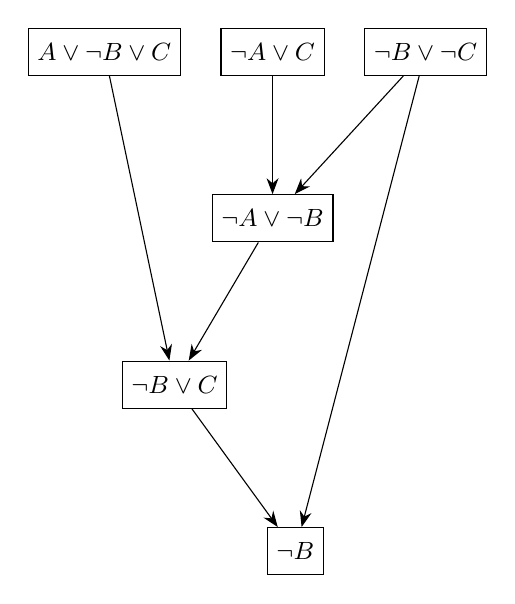
\begin{tikzpicture}[
    node distance=1.5cm and 0.5cm,
    clause/.style={draw, rectangle, minimum height=0.6cm, font=\small},
    arrow/.style={-{Stealth[scale=1.2]}, thin}
]

    \node[clause] (c1) {$A \vee \neg B \vee C$};
    \node[clause, right=of c1] (c3) {$\neg A \vee C$};
    \node[clause, right=of c3] (c2) {$\neg B \vee \neg C$};

    \node[clause, below=of c3] (c4) {$\neg A \vee \neg B$};
    
    \node[clause, below left=1.5cm and -0.2cm of c4] (c5) {$\neg B \vee C$};
    
    \node[clause, below right=1.5cm and 0.5cm of c5] (c6) {$\neg B$};

    \draw[arrow] (c2) -- (c4);
    \draw[arrow] (c3) -- (c4);
    
    \draw[arrow] (c1) -- (c5);
    \draw[arrow] (c4) -- (c5);
    
    \draw[arrow] (c5) -- (c6);
    \draw[arrow] (c2) -- (c6);

\end{tikzpicture}
\end{center}

Potremmo anche fermarci qui senza calcolare $A \vee \neg B$, in quanto $\neg B \models (A \vee \neg B)$.

In ogni caso, segue il grafo delle possibili derivazioni:

\begin{center}
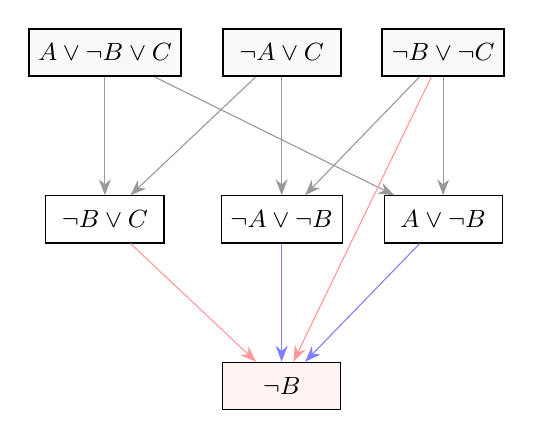
\begin{tikzpicture}[
    node distance=1.5cm and 0.5cm,
    clause/.style={draw, rectangle, minimum height=0.6cm, minimum width=1.5cm, font=\small},
    input/.style={clause, thick, fill=gray!5},
    arrow/.style={-{Stealth[scale=1.2]}, thin, gray!80}
]

    \node[input] (c1) {$A \vee \neg B \vee C$};
    \node[input, right=of c1] (c3) {$\neg A \vee C$};
    \node[input, right=of c3] (c2) {$\neg B \vee \neg C$};

    \node[clause, below=of c1] (c5) {$\neg B \vee C$};      
    \node[clause, below=of c3] (c4) {$\neg A \vee \neg B$}; 
    \node[clause, below=of c2] (c7) {$A \vee \neg B$};    
    
    \node[clause, below=1.5cm of c4, fill=red!5] (c6) {$\neg B$};

    \draw[arrow] (c1) -- (c5);
    \draw[arrow] (c3) -- (c5);
    
    \draw[arrow] (c3) -- (c4);
    \draw[arrow] (c2) -- (c4);

    \draw[arrow] (c1) -- (c7);
    \draw[arrow] (c2) -- (c7);
    
    \draw[arrow, red!40] (c5) -- (c6);
    \draw[arrow, red!40] (c2) -- (c6);
    \draw[arrow, blue!50] (c4) -- (c6);
    \draw[arrow, blue!50] (c7) -- (c6);

\end{tikzpicture}
\end{center}

Poiché si arriva al punto fisso senza ottenere la clausola vuota, la formula è soddisfacibile (un modello è $B = F, \ C = T, \ A = T/F$).

\end{document}
